\section*{Fourierreihen Aufgaben mit L�sungen}\label{MA2-fourierreihen-loesungen}

\ifintegriereaufgaben Erkl�rungen und Beispiele, die zum Verst�ndnis der L�sungswege hilfreich sind, finden Sie im Skript\wennreferenzvorhanden{MA2-fourierreihen}{ (Abschnitt \abschnittsverweis{MA2-fourierreihen})}. \fi

	\begin{exercisebox}[Harmonische Schwingungen]
		Bestimmen Sie die Amplitude, die Periode und die Nullphase der folgenden harmonischen Schwingungen und skizzieren sie den Funktionsverlauf
		\begin{eqnarray*}
		(a)\; y(t) = \textcolor{red}{2\,\sin\left(3\, t-\dfrac{\pi}{6} \right)}\quad \quad (b)\; y(t) = \textcolor{blue}{10\,\sin\left(\pi\, t - 3\,\pi\right)}\,.
		\end{eqnarray*}
\vspace{0.3cm}
\noindent \textbf{L�sung:}
\vspace{0.3cm}

	\begin{minipage}{0.6\textwidth}
	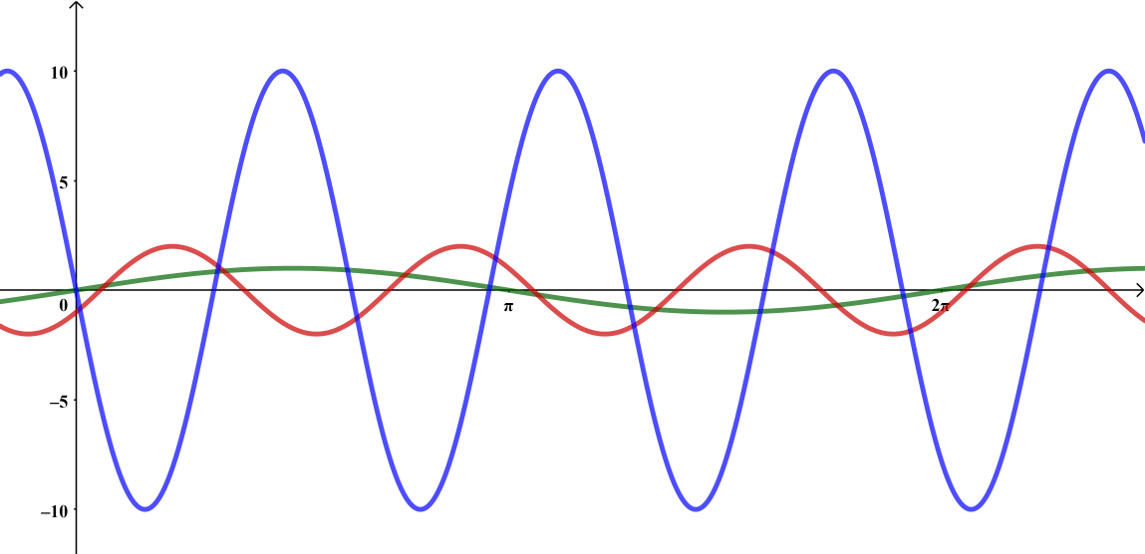
\includegraphics[width=\textwidth]{../Mathematik_2/Bilder/harmonische_schwingungen_amplitude_periode_phase.png}
\end{minipage}
	\begin{minipage}{0.4\textwidth}
		\begin{itemize}
			\item[(a)]  $\textcolor{red}{A=2, \, T= \dfrac{2\pi}{3}, \, \varphi_0 = -\dfrac{\pi}{6} }$
			\item[(b)]  $\textcolor{blue}{A=10, \, T= 2, \, \varphi_0 = -3\pi }$
				\item[(c)] \( \textcolor{darkgreen}{ A=1, \, T= 2\pi, \, \varphi_0 = 0 } \) \newline (Sinus-Funktion zum Vergleich)
\end{itemize}
\end{minipage}

\end{exercisebox}

	\begin{exercisebox}[komplexes Fourier-Polynom vs. reelles Fourier-Polynom]
		\begin{itemize}
			\item[(a)]
		Man kann die komplexwertigen Koffizienten $c_k$ eines komplexen Fourier Polynoms
		\[
			p_{N,f}(t) = \sum\limits_{k=-N}^N c_k\cdot e^{i\,k\,\omega_0\, t} \,,
		\]
		in die reell-wertigen Koeffizienten $a_n$ und $b_n$ des entsprechenden reellen Fourier-Polynom umrechnen und das funktioniert wie folgt:

		\begin{equation}\label{a_k_zu_c_k}
			\left\{ \begin{array}{rcl}
				a_0 & = &  2\, c_0, \\[1ex]
				a_n & = & c_n + c_{-n},\\[1ex]
				b_n & = & i \, \left( c_{-n} + c_{n}\right) \,.
		\end{array}\right.
	\end{equation}
\item[(b)]
		Man kann die reellen Koffizienten eines Fourier Polynoms
		\[
			p_{N,f}(t) = \frac{a_0}{2} + \sum\limits_{n=1}^N\left( a_n\cdot \cos( n \, \omega_0 \, t) + b_n \cdot \sin(n \, \omega_0\, t)\right)\,,
		\]
		in die komplex-wertigen Koeffizienten $c_k$ des entsprechend komplex-wertigen Fourier-Polynoms umrechnen und das funktioniert wie folgt:
		\begin{eqnarray*}
			&& \begin{cases}
				c_0 = \frac12\, a_0,\\[1ex]
				c_n = \frac12\, \left( a_n - i\, b_n\right) , \quad n \in \mathbb N^+\,, \\[1ex]
			c_{-n} = \frac12 \, \left( a_n + i \, b_n\right),\quad  , \quad n \in \mathbb N^+\,. \end{cases}
	\end{eqnarray*}
	\end{itemize}
\end{exercisebox}


\begin{exercisebox}[Fourier-Reihen]
	Skizzieren Sie zun�chst die Funktionen und berechnen Sie anschlie�end die Fourier-Reihen.
	\begin{itemize}
		\item[(a)] Periode $T=2$ und
			\[ f(t) = t, \quad t \in [0,2]\,.\]
		\item[(b)] Periode $T=1$ und
			\[ f(t) = |t|, \quad t \in \left[-\frac12,\frac12\right]\,.\]
		\item[(c)] Periode $T>0$ und
			\[ f(t) = t\cdot (T-t), \quad t \in [0,T]\,.\]
		\item[(d)] Periode $T=2\pi$ und
			\[ f(t) = \max(\sin(t),0), \quad t \in [0,2\pi]\,.\]

	\end{itemize}
\vspace{0.3cm}
\noindent \textbf{L�sung:}

\begin{itemize}
	\item[(a)] Eine Skizze des Signals zeigt, dass \(f\) um die horizontale Gerade \( x\mapsto 1\) schwingt. Aus dieser Beobachtung folgt, dass der konstante Anteil der Fourierreihe, also der Summand \(a_0/2\) bzw. \(c_0\), den Zahlenwert eins hat. Bez�glich des Punkts \( (1|0)\) ist \(f\) punktsymmetrisch und damit ein ungerades Signal. Die Fourierkoeffizienten lauten
		\begin{eqnarray*} \begin{cases} a_0 = 2, \quad &\\
				a_k = 0, \quad &k>0, \\
				b_k = -\displaystyle{\frac{2}{\pi k}}, \quad &k>0\,.
			\end{cases}
		\end{eqnarray*}
		Die Periode \(T\) definiert die Grundfreqzenz \(\omega_0 = \dfrac{2\pi}{T} = \pi\) und damit erhalten wir
		\begin{eqnarray*}
			\mathrm{FR}_f(t) = \frac{a_0}{2} + \sum\limits_{k=1}^\infty a_k\cdot\cos( k\,\omega_0\, t) + b_k\cdot \sin(k\,\omega_0\,t) =  1 - \sum\limits_{k=1}^\infty \frac{2}{k \,\pi} \cdot \sin(k \, \pi \,t) \,.
		\end{eqnarray*}

		\vspace{0.2cm}
		\noindent\textbf{Bemerkung:}
		Entwickelt man anstatt der reellen Fourierreihe die komplexe Fourierreihe, dann kann es sein, dass die Fourierreihen auf den ersten Blick nicht dieselbe Form haben. Entweder kann man die Reihen auf Gleichheit �berpr�fen, indem man �berpr�ft, ob die Umrechnungsformel \eqref{a_k_zu_c_k} wahr sind. Eine Alternative ist die komplexe Reihe in eine reelle Reihe umzuformen. Letzteres klappt wie folgt
		\begin{itemize}
			\item Komplexe Reihe in drei Teile aufspalten \[ \mathrm{FR}_f(t) = \sum\limits_{-\infty}^\infty c_k\cdot e^{i \, k \, \omega_0\,t} = \sum\limits_{k=-\infty}^{k=-1} c_k\cdot e^{i\, k \, \omega_0\, t} + c_0 + \sum\limits_{k=1}^\infty c_k\cdot e^{i \, k\, \omega_0\, t} \]
			\item Summanden der Reihe umsortieren: \[ \mathrm{FR}_f(t) = c_0 + \sum\limits_{k=1}^\infty \left( c_k\cdot  e^{i \, k\,\pi\, t} + c_{-k}\cdot e^{-i \, k \, \pi\, t} \right) \]
			\item Komplex konjugierte Zahlen identifizieren
				\[ \mathrm{FR}_f(t) = c_0 + \sum\limits_{k=1}^\infty \left(  c_k\cdot e^{i \, k\,\pi\, t} + \overline { c_{k} \cdot e^{i \, k\, \pi \, t} } +\right)\,, \] wobei
				\begin{eqnarray*} c_{-k} &=& \overline{ c_k} \,,\\ e^{-i \, k\,\omega_0\, t} &=& \overline{ e^{i \, k \omega_0\, t} }\,, \\\Rightarrow c_{-k}\cdot e^{-i\, k\, \omega_0\, t} &=& \overline{ c_k \cdot e^{i \, k \,\omega_0\,t}}\,.\end{eqnarray*}
			\item Reelle und imagin�re Anteile trennen und Eulersche Identit�ten
				\begin{eqnarray*}
					\cos\left(k\, \omega_0\, t\right) &=& \frac12\cdot \left( e^{i\, k\,\omega_0\, t} + e^{-i\, \, k \, \omega_0\,t} \right) \,,\\
				\sin\left( k \, \omega_0 \, t\right) &=& -\frac{i}{2}\, \left( e^{i\, k\,\omega_0\,t } - e^{-i\, \, k\,\omega_0\,t } \right) \,.\end{eqnarray*}

				anwenden.
		\end{itemize}
	\item[(b)] $f$ ist achsensymmetrisch (gerade) mit Periode \(T = 1\), also Grundschwingung \(\omega_0 = \dfrac{2\pi}{T} = 2\pi\) . Die Fourierkoeffizienten sind
		\begin{eqnarray*} \begin{cases} a_0 &= \displaystyle{\frac12}\,,\\
				a_k &= \displaystyle{\frac{(-1)^k - 1 }{\pi^2 k^2} } = \begin{cases} 0,  &\quad k \; \textnormal{gerade}, \\ \displaystyle{\frac{-2}{\pi^2 k^2} }, & \quad k \; \textnormal{ungerade}\,,\end{cases}\\
				b_k &= 0\,, \quad \textnormal{f�r alle } k\geq 1\,.
			\end{cases}
			\end{eqnarray*}
			Die Funktion l��t sich also allein durch Kosinus-Schwingungen rekonstruieren, alle \(b_k\) sind null. Weiterhin tauchen nur Frequenzen auf mit ungeradem Index:  \[a_{2k-1}= - \dfrac{2}{\pi^2 ( 2k-1)^2}, \quad k = 1,\cdots \,.\]
			\begin{eqnarray*}
				\Rightarrow\quad  \mathrm{FR}_f(t) &=& \dfrac{a_0}{2} + \sum\limits_{k=1}^\infty a_k\cdot \cos\left( k \, \omega_0\, t\right) + b_k\cdot \sin\left( k \,\omega_0\, t\right) \\
				&=& \dfrac14 + \sum\limits_{k=1}^\infty \dfrac{-2}{\pi^2\,(2\,k-1)^2} \cdot \cos(2\pi\,(2\,k-1)\, t) \\
				&=& \frac14 - \frac{2}{\pi^2} \left( \frac{\cos(2\pi\, t)}{1^2} + \frac{\cos(3\cdot 2\pi\, t)}{3^2} + \frac{\cos(5\cdot 2\pi\, t)}{5^2} + \dots \right)
		\end{eqnarray*}
	\item[(c)] $f$ ist achsensymmetrisch (gerade) mit Periode \(T\) und Grundschwingung \(\omega_0 = \dfrac{2\pi}{T}\). Die Fourierkoeffizienten lauten
		\begin{eqnarray*}
			\begin{cases} a_0 = \displaystyle{\frac{T^2}{3}}, \quad &\\
				a_k = -\displaystyle{\frac{T^2 }{\pi^2 k^2} }, \quad &k>0, \\
				b_k = 0, \quad &k>0\,.
			\end{cases}
			\end{eqnarray*}
			\begin{eqnarray*}
				\Rightarrow\quad \mathrm{FR}_f(t) &=& \frac{T^2}{6} - \frac{T^2}{\pi^2} \sum\limits_{k=1}^\infty \frac{1}{k^2} \cos\left(k \, \omega_0\,t\right) \\
				&=& \frac{T^2}{6} - \frac{T^2}{\pi^2}\cdot \left( \frac{\cos(\omega_0\, t)}{1^2} + \frac{\cos(2\cdot \omega_0\, t)}{2^2} + \frac{\cos(3\cdot \omega_0\, t)}{3^2} + \dots \right)
		\end{eqnarray*}
	\item[(d)] $f$ ist \(\pi\)-periodisch und weder gerade noch ungerade. Die Fourierkoeffizienten lauten
		\begin{eqnarray*}
			\begin{cases} a_0 = \displaystyle{\frac{2}{\pi}}, \quad &\\
				a_k = -\displaystyle{\frac{(-1)^k+1 }{\pi k^2 -\pi} }, \quad &k>0, \\
				b_1 = \displaystyle{\frac12} \,, & \\
				b_k = 0 \,, & k>1
			\end{cases}
			\end{eqnarray*}
			\begin{eqnarray*}
				\omega_0 = 2\; \Rightarrow\quad \mathrm{FR}_f(t) &=& \frac{1}{\pi} + \frac{1}{2}\sin(t) + \frac{2}{\pi}\cdot \sum\limits_{k=1}^\infty \frac{1}{(2k)^2-1 }\cdot \cos\left(2\,k\, t\right) \\
				&=& \frac{1}{\pi} + \frac{1}{2}\cdot \sin(t) + \frac{2}{\pi}\cdot \left( \frac{\cos(2 \,t)}{2^2-1} + \frac{\cos(4\, t)}{4^2-1} + \frac{\cos(6\, t)}{6^2-1} + \dots \right)
		\end{eqnarray*}
	\end{itemize}
\end{exercisebox}


%\begin{exabox}{\hyperlink{Aufabe_8.6}{Interpolationseigenschaft}}{ }
%Um uns davon zu �berzeugen, setzen wir \(\tilde c_k\) ein,
%\begin{eqnarray*}
%	g_n(t_j) &=& \dfrac{1}{n} \sum\limits_{k=0}^{n-1} \tilde c_k e^{i k \omega_0 t_j } \\[2ex]
%	%&=& \sum\limits_{k=0}^{n-1} \textcolor{blue}{\tilde c_k} e^{i k \, 2\pi/(n\cdot h)\, j\cdot h }\\[2ex]
%	&=& \sum\limits_{k=0}^{n-1} \textcolor{blue}{\tilde c_k} e^{i k \, 2\pi/n\, j } \\[2ex]
%	&=& \sum\limits_{k=0}^{n-1}  \textcolor{blue}{ \dfrac1n \sum\limits_{l=0}^{n-1} f_l \cdot e^{-i \, k\, 2\pi\, l/n} } e^{i k \, 2\pi/n\, j } \\[2ex]
%	&=& \textcolor{blue}{\dfrac{1}{n} \sum\limits_{l=0}^{n-1} f_l} \sum\limits_{k=0}^{n-1} \textcolor{blue}{ e^{-i \, k\, 2\pi\, l/n} } e^{i k \, 2\pi/n\, j } \\[2ex]
%	&=& \dfrac{1}{n} \sum\limits_{l=0}^{n-1} f_l \sum\limits_{k=0}^{n-1} e^{i 2\pi\, (j-l)k/ n} \\[2ex]
%	&\stackrel{(*)}{=}& \dfrac{1}{n} \sum\limits_{l=0}^{n-1} f_l \cdot n \cdot \delta_{lj} \\[2ex]
%	&=& f_j\,.
%\end{eqnarray*}
%\((*)\) folgt aus der folgenden Beobachtung:
%\[ \sum\limits_{k=0}^{n-1} e^{i \,2\pi (j-l) k/n} = \sum\limits_{k=0}^{n-1} \left( z^{j-l}\right)^k = n\cdot \delta_{jl} = \begin{cases} n,\quad j= l\,,\\ 0,\quad j\not=l\,, \end{cases} \]
%	wobei sich das letzte Ergebnis im Detail wie folgt zeigen l��t
%	\begin{itemize}
%		\item f�r \(j=l\) wird der Exponent in jedem Summand null und damit \[\sum\limits_{k=0}^{n-1} z^{0\cdot k} = \sum\limits_{k=0}^{n-1} 1 = n\,.\]
%		\item f�r \(j\not=l\) ist der Wert der Summe null. Die \(n\)-te Potenz einer beliebigen Einheitswurzel \(Z\) ist eins und damit
%			\[ \sum\limits_{k=0}^{n-1} Z^k = 1 + Z + Z^2 + \cdots + Z^{n-1} = \dfrac{ Z^n -1}{Z-1} = \dfrac{1-1}{Z-1} = 0\,.\]
%	\end{itemize}
%
%	Wenn man f�r ein gegebenes diskretes Spektrum die Messwerte des Signals berechnet, f�hrt invertiert man quasi den Zerlegungsprozess. Man nennt das Verfahren die inverse Diskrete Fouriertransformation [iDFT].
%	Zusammen lauten die Formeln
%	\begin{eqnarray*}
%		\textnormal{DFT:}\quad \{f_j\}_{j=0}^{n-1} &\mapsto& \{\tilde c_j\}_{j=0}^{n-1}\,, \\
%		\tilde c_j &=& \dfrac{1}{n} \sum\limits_{k=0}^{n-1} f_k e^{- i \, k 2\pi \,j/n}\,, \quad j=0,\cdots,n-1\,,\\
%		\textnormal{iDFT:}\quad \{\tilde c_j\}_{j=0}^{n-1} &\mapsto& \{f_j\}_{j=0}^{n-1}\,, \\
%		f_j &=& \sum\limits_{k=0}^{n-1} \tilde c_k e^{i \, k 2\pi \,j/n}\,, \quad j=0,\cdots,n-1\,.
%	\end{eqnarray*}
%\end{exabox}


